% PART VI — WEB-BASED SIMULATION CONTROL CENTER
\chapter{Chapter 9: Refactored Robotics Workstation, FastAPI Core, and Three.js Digital Twin}
\section{9.1 Authoritative PyBullet-to-Browser Architecture}
Following Phase 0 repository auditing (`docs/repository\_audit.md`, pinning `backup/pre-restructure-ph17`, archiving 41 loose root scripts into `archive/historical/root\_scripts/`), the project added a restrained dark industrial web workstation under `backend/` and `frontend/`. Crucially, PyBullet remains the single authoritative source of truth (Figure 9.1): a thread-safe `SimulationManager` steps PyBullet at 20 Hz and streams 11 real `panda.urdf` link frame transforms, cube/peg poses, sorting bins, and trajectory coordinates via WebSocket `/ws/simulation`. React Three Fiber renders official `.obj`/`.mtl` Panda geometry via `OBJLoader` + `MTLLoader` strictly from streamed physics frames — never running client-side forward kinematics animations that could diverge from simulation truth.

\begin{figure}[htbp]\centering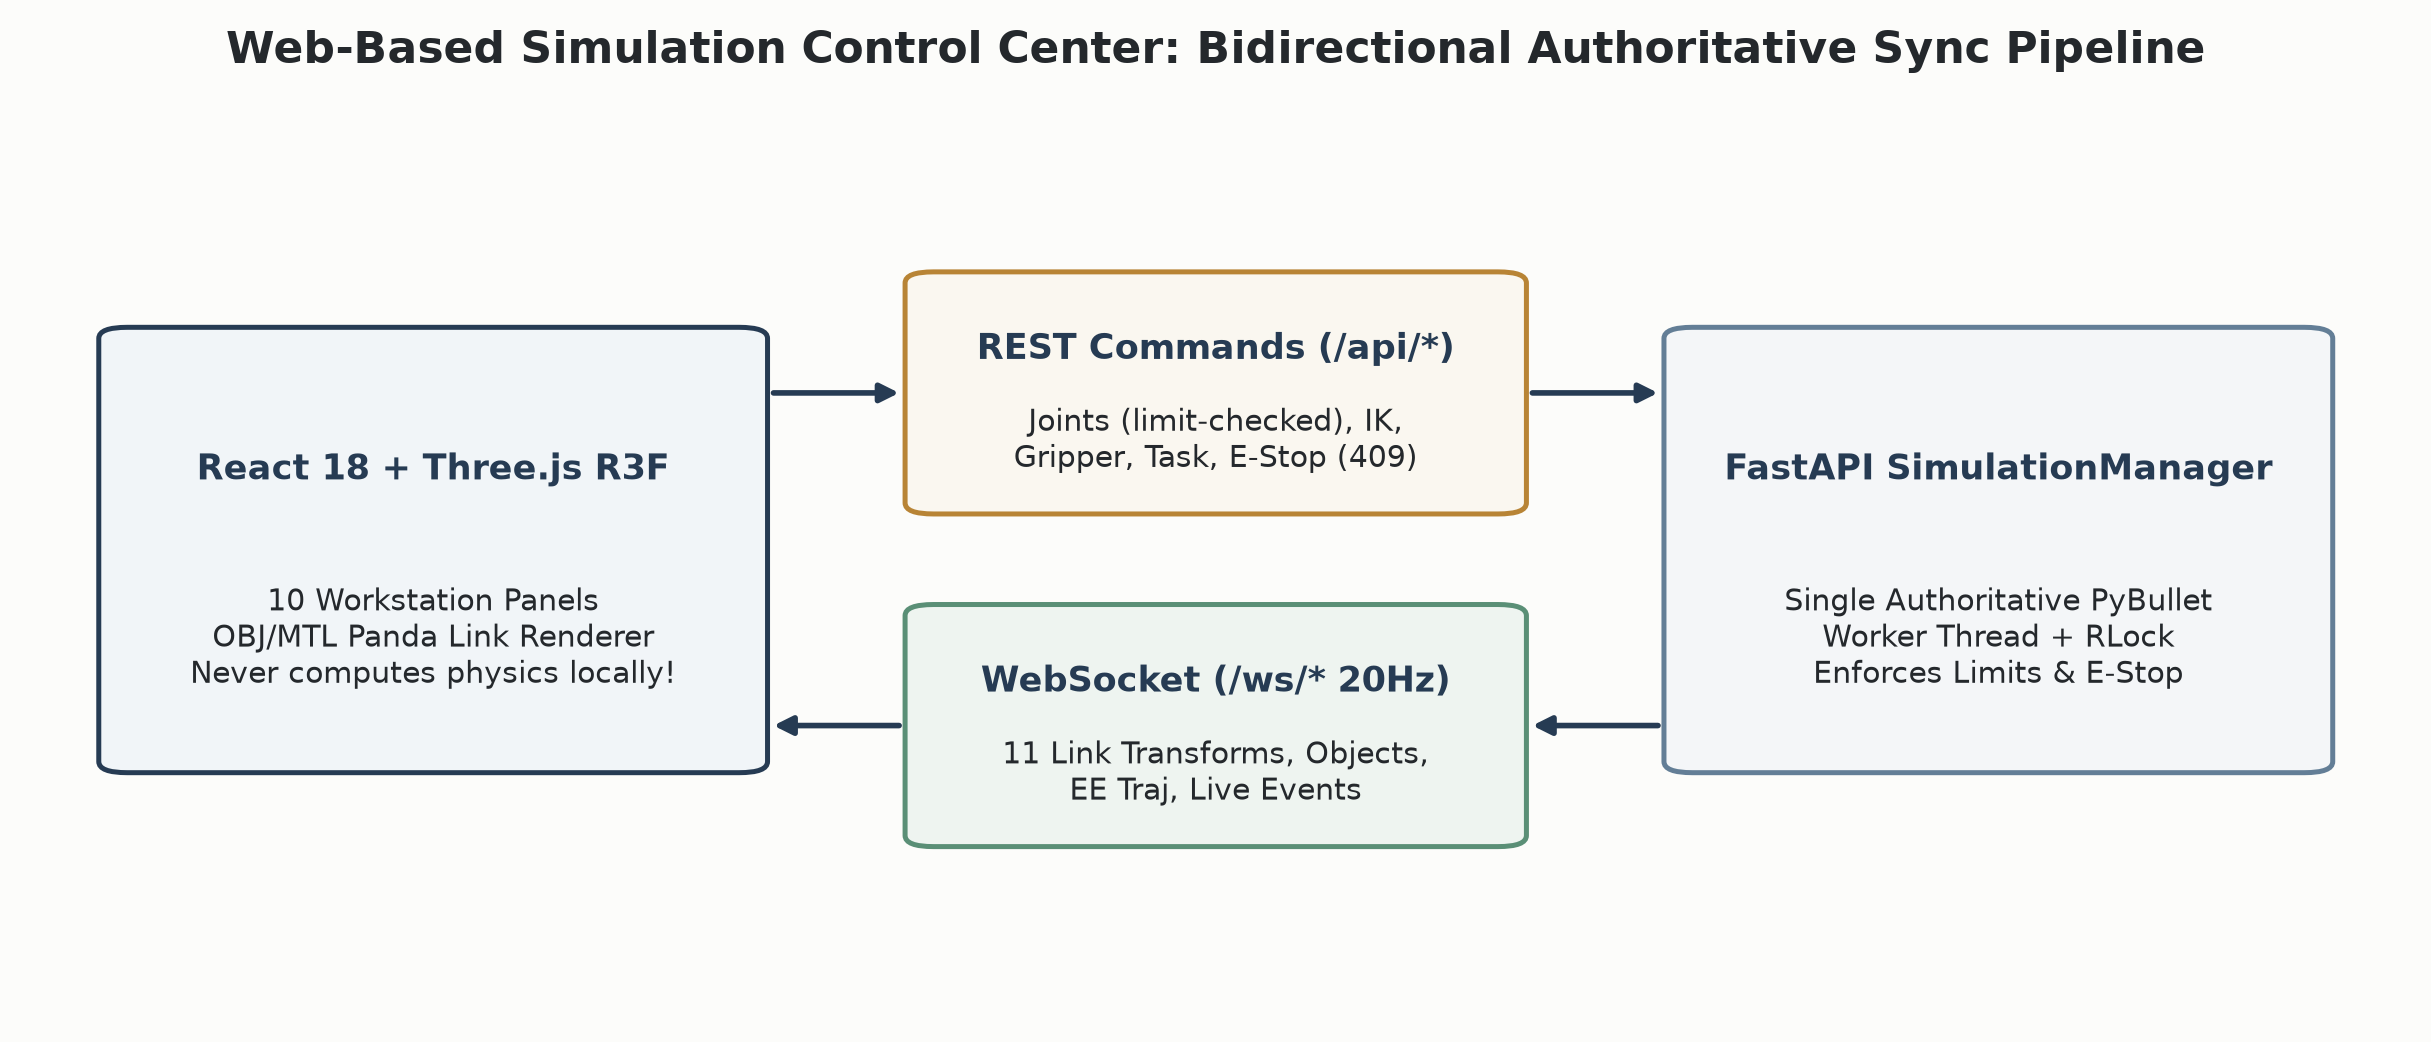
\includegraphics[width=0.9\linewidth]{../../assets/diagrams/diag_12_website_websocket_architecture.png}\caption{Figure 9.1: Authoritative FastAPI SimulationManager, REST validation gates, 20 Hz WebSocket stream, and Three.js renderer.}\end{figure}
\begin{figure}[htbp]\centering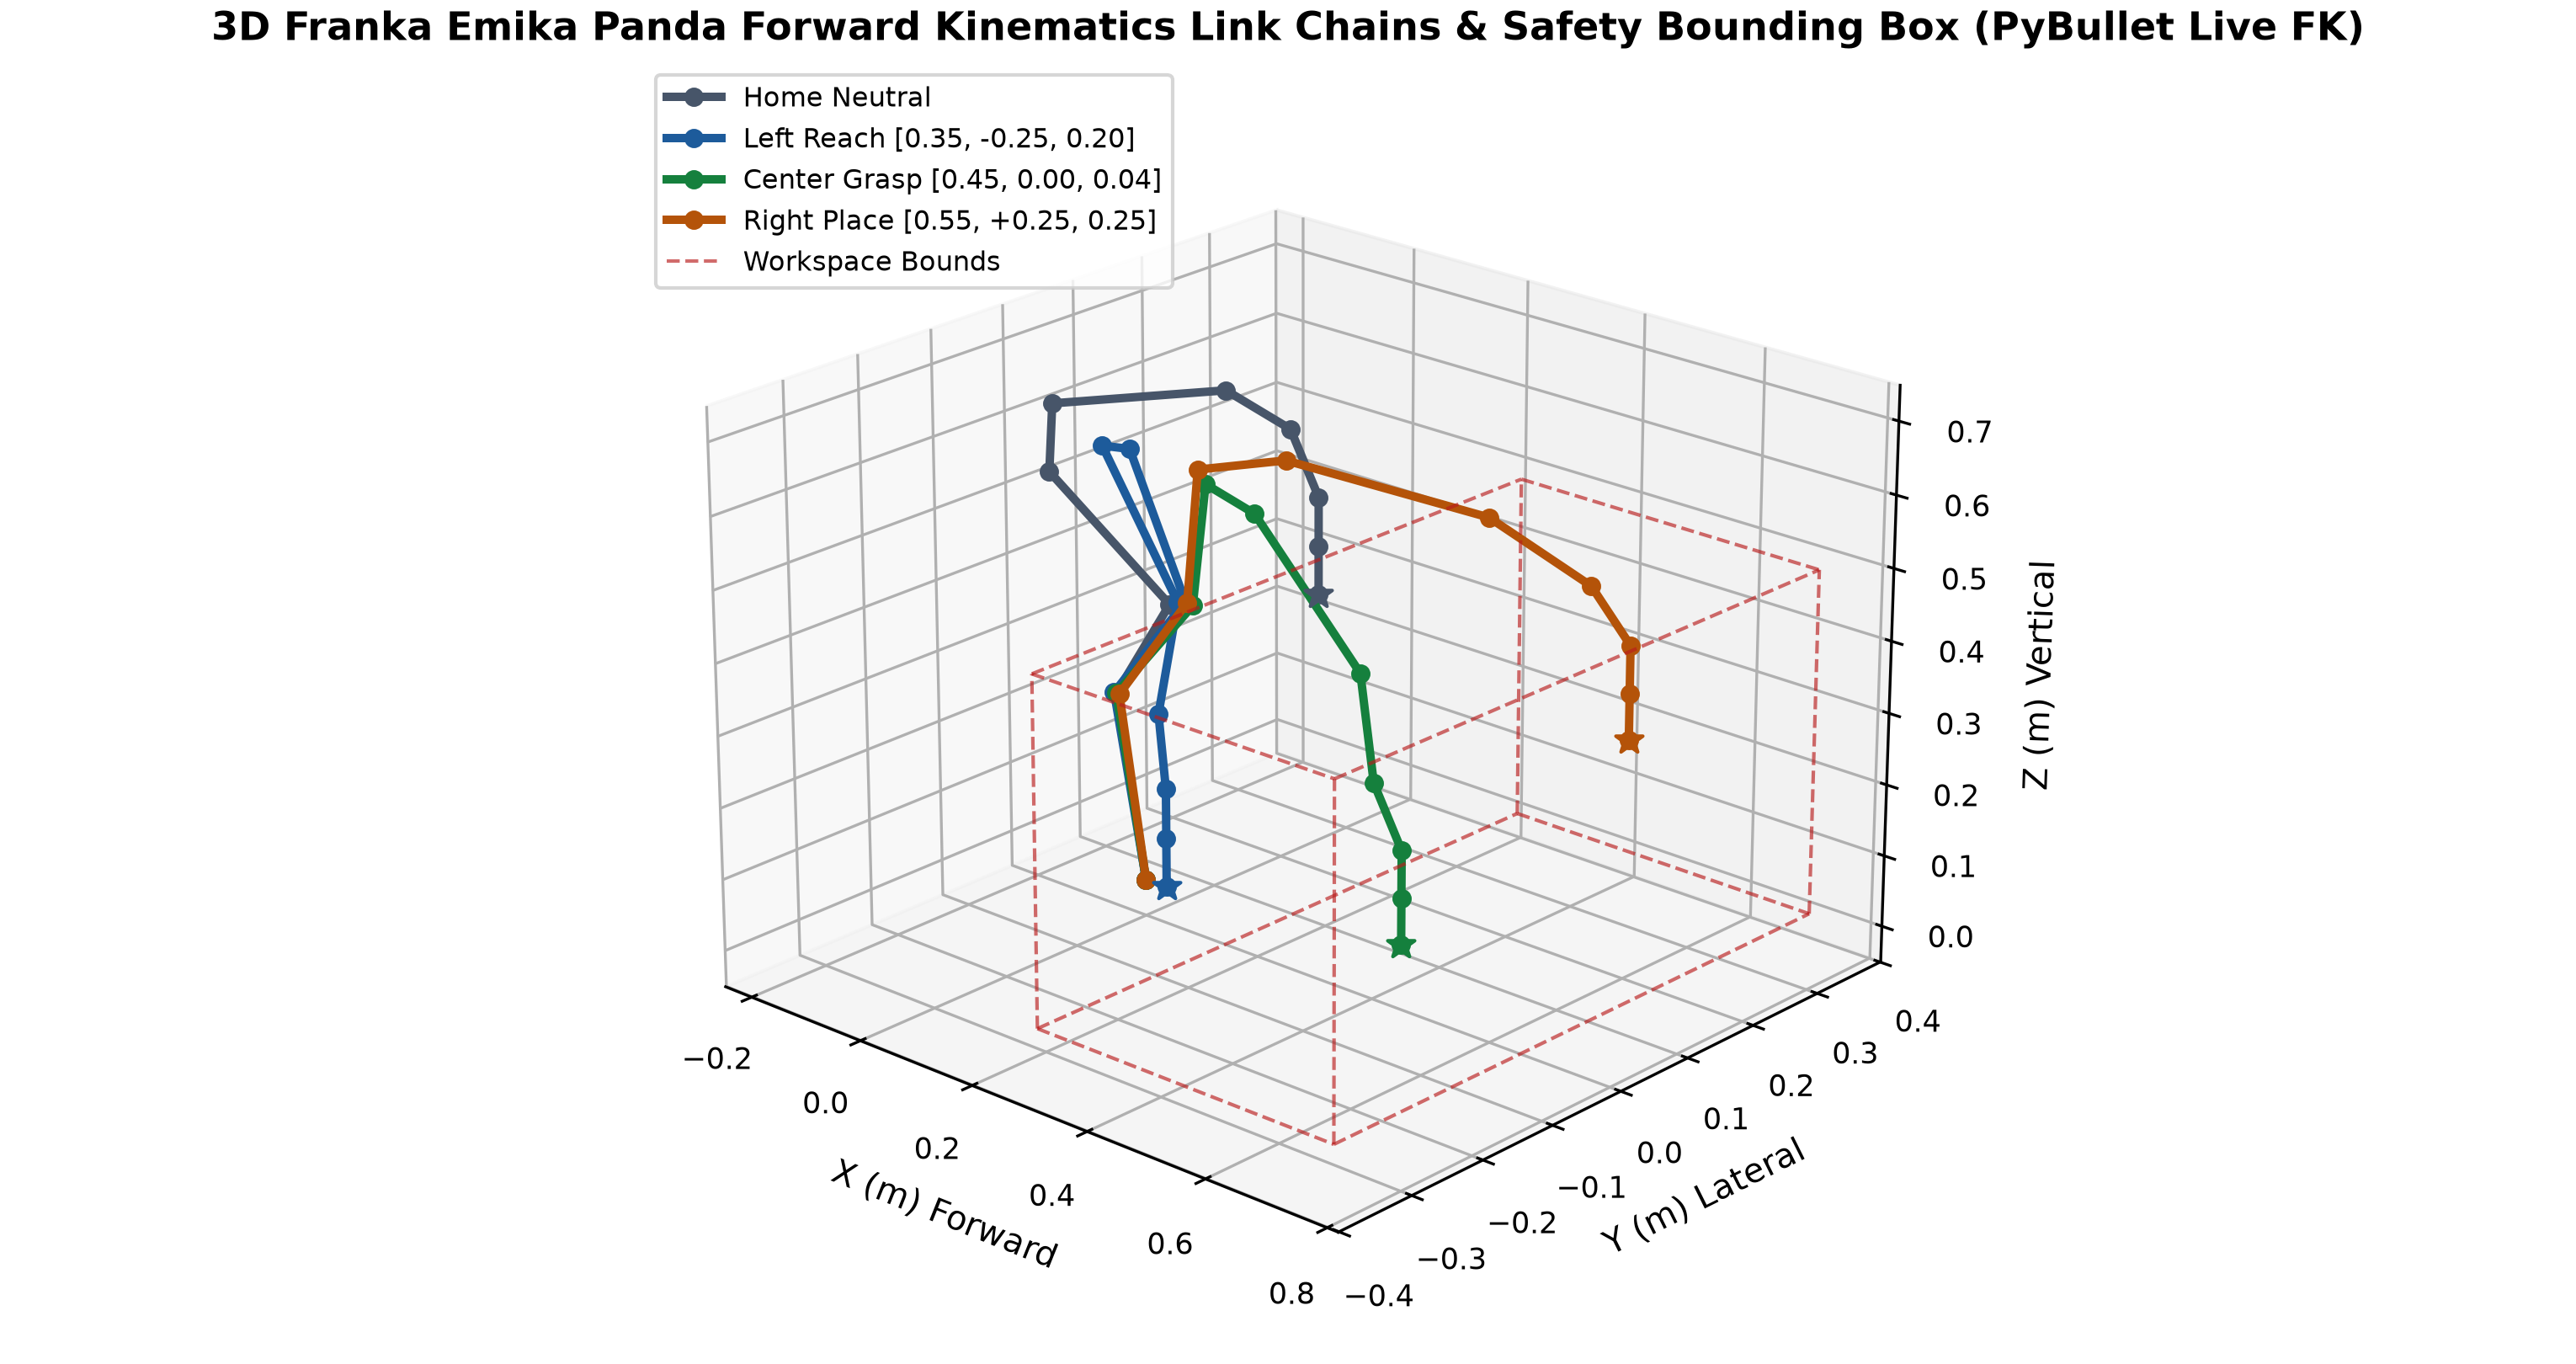
\includegraphics[width=0.9\linewidth]{../../assets/plots/plot_10_panda_3d_fk_and_rgbd_cloud.png}\caption{Figure 9.2: Three-dimensional workspace bounds and multi-target Panda kinematic chains mirrored between PyBullet and workstation.}\end{figure}
\section{9.2 Implemented Web Controls, Task Verification \& Known Limits}
Verified functionality (`126` combined Python + backend integration tests, `tsc -b \&\& vite build`, and `2/2` Vitest UI checks): (i) 7-DOF joint sliders enforcing `panda.urdf` radian limits (`HTTP 422` on violations); (ii) Cartesian `(X, Y, Z, Roll, Pitch, Yaw)` command resolution via `FrankaPanda.calculate\_ik` displaying requested vs. achieved pose and millimeter tracking error; (iii) Parallel-jaw gripper open/close/width actuation; (iv) Operator E-Stop halting active tasks and locking motors (`HTTP 409` until reset); (v) Live task runner (`reach\_target`, `pick\_lift`, `pick\_place`, `multi\_sort`, `assembly\_insert`, `dynamic\_manip`, returning `HTTP 501` for unimplemented physical FCI); and (vi) Experiment \& Evaluation browser (`experiment\_inventory.csv` + CSV export + Recharts). Known limitation: interactive live Chromium browser WebGL rendering validation remains manual startup verification rather than headless Playwright CI.
